% !TEX root = main.tex

\section{深层网络训练的挑战} % ch8.7.1
\subsection{过拟合}
提升模型泛化能力的几种方法:
\begin{itemize}
    \item 数据集分划:训练集60\%、验证集20\%、测试集20\%
    \item 早停(early stopping):验证集误差不再下降时
    \item 规范化(regularization)
    \[\mL(\vtheta)=\frac{1}{N}\mL(\vy_n,\vf(\vx_n;\vtheta))+\lambda\norm{\vtheta}_p\]
    \begin{itemize}
        \item $p=2$:权重衰减(weight decay)/岭回归(ridge),更小的权重值
        \item $p=1$:更少的非零权重
    \end{itemize}
    \item Dropout:训练时某一神经元只有$p$概率出现
    \begin{figure}[H]
        \centering
        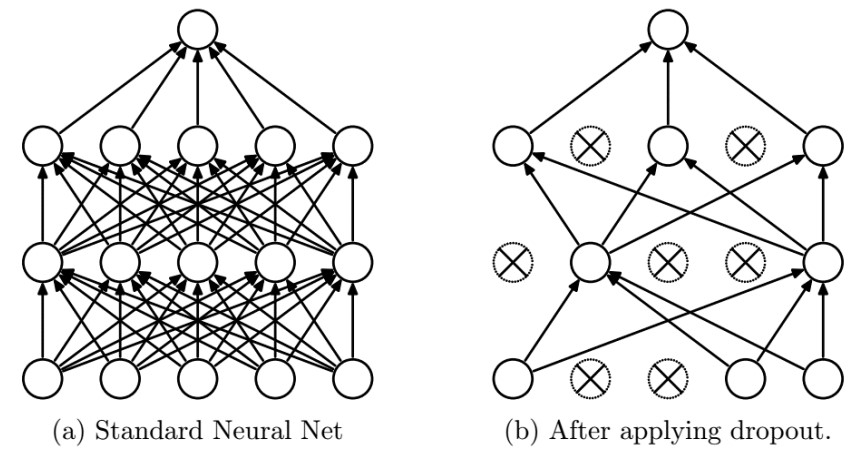
\includegraphics[width=0.6\linewidth]{fig/dropout.jpg}
        \caption{Dropout示意图}
    \end{figure}
    \item 数据增量(augmentation):对原始图片做变换
    \item 集成学习(ensemble)
\end{itemize}

\subsection{梯度问题}
由反向传播算法
\[\begin{aligned}
\pd{\mL}{\layer{W}{1}}
&=\pd{\mL}{\layer{\va}{n_l}}\cdot\lrp{\pd{\layer{\va}{n_l}}{\layer{\vz}{n_l}}\cdot\pd{\layer{\vz}{n_l}}{\layer{\va}{n_l-1}}}\cdot\cdots\cdot\lrp{\pd{\layer{\va}{1}}{\layer{\vz}{1}}\cdot\pd{\layer{\vz}{1}}{\layer{W}{1}}}\\
&=\pd{\mL}{\layer{\va}{n_l}}\cdot\lrp{h'(\layer{\vz}{n_l})\cdot\layer{W}{n_l}}\cdots \lrp{h'(\layer{\vz}{1})\cdot\vx}
\end{aligned}\]
\begin{itemize}
\item 若每一$|h'(\layer{\vz}{l})\layer{W}{l}|>1$,那么相乘起来就会造成梯度爆炸(exploding)
\item 若每一$|h'(\layer{\vz}{l})\layer{W}{l}|<1$,那么相乘起来就会造成梯度消失(vanishing)
\end{itemize}

\subsubsection{梯度爆炸}
令$|h'(\layer{\vz}{l})|\leq 1$且$|\layer{W}{l}|\leq 1$
\begin{itemize}
	\item 对于Sigmoid、Tanh和ReLU来说,$|h'(\layer{\vz}{l})|\leq 1$
	\item 权重初始化,使$|\layer{W}{l}|\leq 1$
	\item 权重重归一(re-normalization) %  https://arxiv.org/abs/1602.07868
\end{itemize}

\subsubsection{梯度消失}
\begin{itemize}
	\item 用ReLU,$\layer{\vz}{l}>0$时,梯度恒为$1$
	\item 如果$W_i$的方差不小,则大多$|W_i|$都不会靠近$0$
	\item 权重初始化:$\layer{W}{l}\thicksim N(0,\sigma^2)$或$\layer{W}{l}\thicksim U(-a,a)$
	\item 权重重归一
\end{itemize}

\subsection{权重初始化}
\subsubsection{Xavier初始化}
希望前向传播输入通过网络层后不收缩(shrink)或爆炸,假设当$\layer{\vz_k}{l}$较小时,$h(\layer{\vz_k}{l})$近似线性,则
\[\layer{\va_k}{l}=h(\layer{\vz_k}{l})
=h\lrp{\sum_{j=1}^n\layer{\va_j}{l-1}\layer{W_{jk}}{l}}
\approx\sum_{j=1}^n\layer{\va_j}{l-1}\layer{W_{jk}}{l}\]
目标是保证输入输出的\textbf{差异性}\footnote{如果没有差异,比如说权重初始化全为$0$,那反向传播算法根本没法工作},又让模型稳定快速收敛。

如何衡量差异性?常用指标即\textbf{方差}。
假设输入信号$\layer{\va_j}{l-1}$和权重参数$W_{jk}$都相互独立、均匀分布且有零均值,那么
\begin{align}
\Var{\layer{\va_k}{l}}
&=\sum_{j=1}^n\Var{\layer{\va_j}{l-1}\layer{W_{jk}}{l}}\\
&=\sum_{j=1}^n\lrp{\E{\lrp{\layer{\va_j}{l-1}\layer{W_{jk}}{l}}^2}-\E{\layer{\va_j}{l-1}\layer{W_{jk}}{l}}^2}\\
&=\sum_{j=1}^n\lrp{\E{\layer{\va_j}{l-1}^2}\E{\layer{W_{jk}}{l}^2}-\E{\layer{\va_j}{l-1}}^2\E{\layer{W_{jk}}{l}}^2}\label{equ:var}\\
&=\sum_{j=1}^n\lrp{\lrp{\Var{\layer{\va_j}{l-1}}+\E{\layer{\va_j}{l-1}}^2}\lrp{\Var{\layer{W_{jk}}{l}}+\E{\layer{W_{jk}}{l}}^2}-\E{\layer{\va_j}{l-1}}^2\E{\layer{W_{jk}}{l}}^2}\\
&=\sum_{j=1}^n\lrp{\Var{\layer{\va_j}{l-1}}\Var{\layer{W_{jk}}{l}}+\Var{\layer{\va_j}{l-1}}\E{\layer{W_{jk}}{l}}^2+\E{\layer{\va_j}{l-1}}^2\Var{\layer{W_{jk}}{l}}}\\
&\approx\sum_{j=1}^n\Var{\layer{\va_j}{l-1}}\Var{\layer{W_{jk}}{l}}\qquad\mbox{零均值}\\
&\approx n\Var{\layer{\va}{l-1}}\Var{\layer{W}{l}}\qquad\mbox{独立同分布}
\end{align}

神经网络实际上是将\textbf{样本空间映射到类别空间}\footnote{参考知乎夕小瑶的文章 - \href{https://zhuanlan.zhihu.com/p/27919794}{深度前馈网络与Xavier初始化原理}},如果样本空间和类别空间的分布差异很大,如类别空间特别稠密,而样本空间特别稀疏,则类别空间用于反向传播的误差返回样本空间显得微不足道,训练会十分缓慢;而如果类别空间特别稀疏,样本空间特别稠密,那么类别空间计算出来的误差返回样本空间将造成极大波动,导致模型发散震荡。
因此应尽可能让样本空间和类别空间的分布差异不要太大,也即令它们的方差尽可能相等,即$\Var{\layer{\va}{l}}\approx\Var{\layer{\va}{l-1}}$,可得
\[\Var{\layer{W}{l}}=\frac{1}{n_{in}}\]

类似地,同样希望反向传播时梯度方差通过网络层时不改变,可以得到
\[\Var{\layer{W}{l}}=\frac{1}{n_{out}}\]

通常输入与输出神经元数目不同,那么取平均得到
\[\Var{\layer{W}{l}}=\frac{2}{n_{in}+n_{out}}\]
故我们得到了Xavier初始化\cite{xavier:ini_2010},可以从高斯分布中采样
\[W\thicksim \mN\lrp{0,\frac{2}{n_{in}+n_{out}}}\]
或者从均匀分布中采样(将均匀分布的方差$\Var{\layer{W}{l}}=(b-a)^2/12$代入求解)
\[W\thicksim \mU\lrp{-\frac{\sqrt{6}}{\sqrt{n_{in}+n_{out}}},\frac{\sqrt{6}}{\sqrt{n_{in}+n_{out}}}}\]

\subsubsection{Kaiming初始化}
但Xavier并不适用于ReLU激活函数,因其假定$\layer{\va}{l}$有零均值,但显然ReLU的输出并没有零均值,因此有了何凯明的方法\cite{kaiming:ini_iccv_2015}。

由公式(\ref{equ:var})及$\E{\layer{W_{jk}}{l}}=0$可得
\[\Var{\layer{\va_k}{l}}=n\Var{\layer{W_{jk}}{l}}\E{\layer{\va_j}{l-1}^2}\]
接下来计算
\[\begin{aligned}
\E{\layer{\va_j}{l-1}^2}
&=\intabu{-\infty}{\infty}{\layer{\va_j}{l-1}^2\pr{\layer{\va_j}{l-1}}}{\layer{\va_j}{l-1}}\\
&=\intabu{-\infty}{\infty}{\max(0,\layer{\vz_j}{l-1})^2\pr{\layer{\vz_j}{l-1}}}{\layer{\vz_j}{l-1}}\qquad\mbox{ReLU}\\
&=\intabu{0}{\infty}{\layer{\vz_j}{l-1}^2\pr{\layer{\vz_j}{l-1}}}{\layer{\vz_j}{l-1}}\\
&=\frac{1}{2}\intabu{-\infty}{\infty}{\layer{\vz_j}{l-1}^2\pr{\layer{\vz_j}{l-1}}}{\layer{\vz_j}{l-1}}\qquad\mbox{假设输出对称分布}\\
&=\frac{1}{2}\Var{\layer{\vz_j}{l-1}}
\end{aligned}\]
进而
\[\Var{\layer{\vz_k}{l}}=\frac{\layer{n}{l}}{2}\Var{\layer{W_{jk}}{l}}\Var{\layer{\vz_j}{l-1}}\]
迭代得到
\[\Var{\layer{\vz}{n_l}}=\Var{\layer{\vz}{1}}\lrp{\prod_{l=2}^{n_l}\frac{\layer{n}{l}}{2}\Var{\layer{W}{l}}}\]
令$\Var{\layer{\vz}{n_l}}=\Var{\layer{\vz}{1}}$,有
\[\frac{\layer{n}{l}}{2}\Var{\layer{W}{l}}=1,\;\forall l\]
最终得到高斯分布采样
\[W\thicksim \mN\lrp{0,\frac{2}{\layer{n}{l}}}\]
或者从均匀分布中采样
\[W\thicksim \mU\lrp{-\sqrt{\frac{6}{\layer{n}{l}}},\sqrt{\frac{6}{\layer{n}{l}}}}\]

\subsection{归一化}
\subsubsection{批归一化}
不同批次可能有不同的分布,导致梯度下降难收敛,因此希望使输入的批次都有相似的分布,于是就有了批归一化(batch normalization, BN)技术\cite{ioffe:bn_2015}。

对于每一个批$\{\smp{\vx}{i}\}$,归一化每一个维度
\[\hat{\vx}_k=\frac{\vx_k-\E{\vx_k}}{\sqrt{\Var{\vx_k}+\eps}}\]
但直接这样做会降低神经元的表达力,因此要恢复其多样性/非线性性
\[\tilde{\vx}_k=\gamma_k\hat{\vx}_k+\beta_k\equiv \mathrm{BN}_{\gamma_k,\beta_k}(\vx_k)\]
其中$\gamma_k$和$\beta_k$与每个批次数据独立,不同维度有不同$\gamma_k$和$\beta_k$。
为了确定每个神经元的$\gamma_k$和$\beta_k$,则可以将其作为参数进行训练。

\subsubsection{组归一化}
批归一化可以实现更快的收敛速度及更高的精度,但批归一化不能对小的批次大小起作用(如批大小为$4$)。
组归一化(group normalization, GN)\cite{he:gn_2018}则将通道划分为组,然后在每个组内做归一化,这可以对单一数据起作用。

各种归一化技术的比较可见图\ref{fig:normalization}。
\begin{figure}[H]
\centering
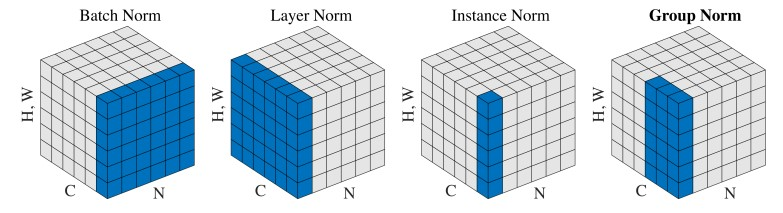
\includegraphics[width=0.8\linewidth]{fig/normalization.jpg}
\caption{批训练归一化技术}
\label{fig:normalization}
\end{figure}

\subsection{更深的网络}
随着神经网络层的增加,训练和测试误差反倒会增加\cite{he:identity_resnet_2016},优化的难度也会越大。

因此尝试用网络学习\textbf{残差映射},而不是直接学习目标映射,此即ResNet\cite{he:resnet_2016}的思想。
\begin{figure}[H]
\centering
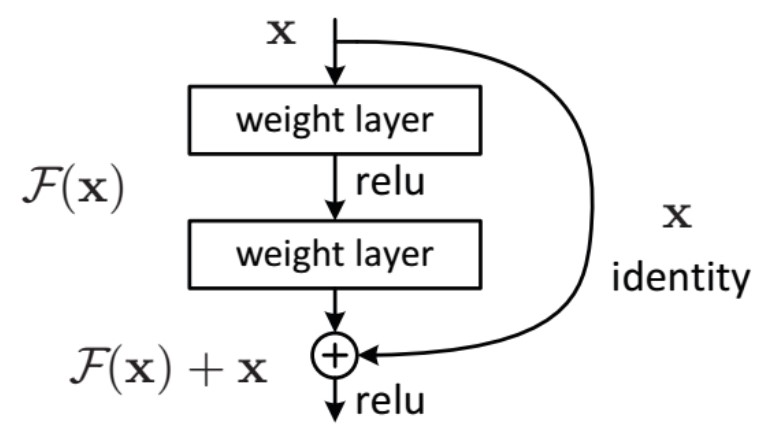
\includegraphics[width=0.5\linewidth]{fig/residual_block.jpg}
\caption{残差模块}
\end{figure}
\[\begin{aligned}
\mathcal{H}(\vx) &= \mF(\vx)+\vx\\
\mF(\vx) &= \mathcal{H}(\vx)-\vx
\end{aligned}\]

ResNet在ImageNet数据集上首次超过人类水平,之后出现了大量拓展,包括DenseNets\cite{huang:densenet_2017}、ResNeXt\cite{xie:resnext_2017}、SENet\cite{hu:senet_2018}、PNASNet\cite{liu:pnasnet}等。